\section{Sharing Reduction}

A key design goal for the implementation of fission was that
communication between producers and consumers of the stream graph be
efficient.  Often when data parallelism is applied, the producer
filter is fissed by the same factor as the consumer filter.  To make
this common case efficient, general graph fission communicates a large
number of items between disjoint producer-consumer pairs of products
of the fission.  Next, a small number of items (the number of items
inspected by the consumer filter) is duplicated and communicated from
producer to a consumer in a different pair.

\begin{figure*}[t]
\centering
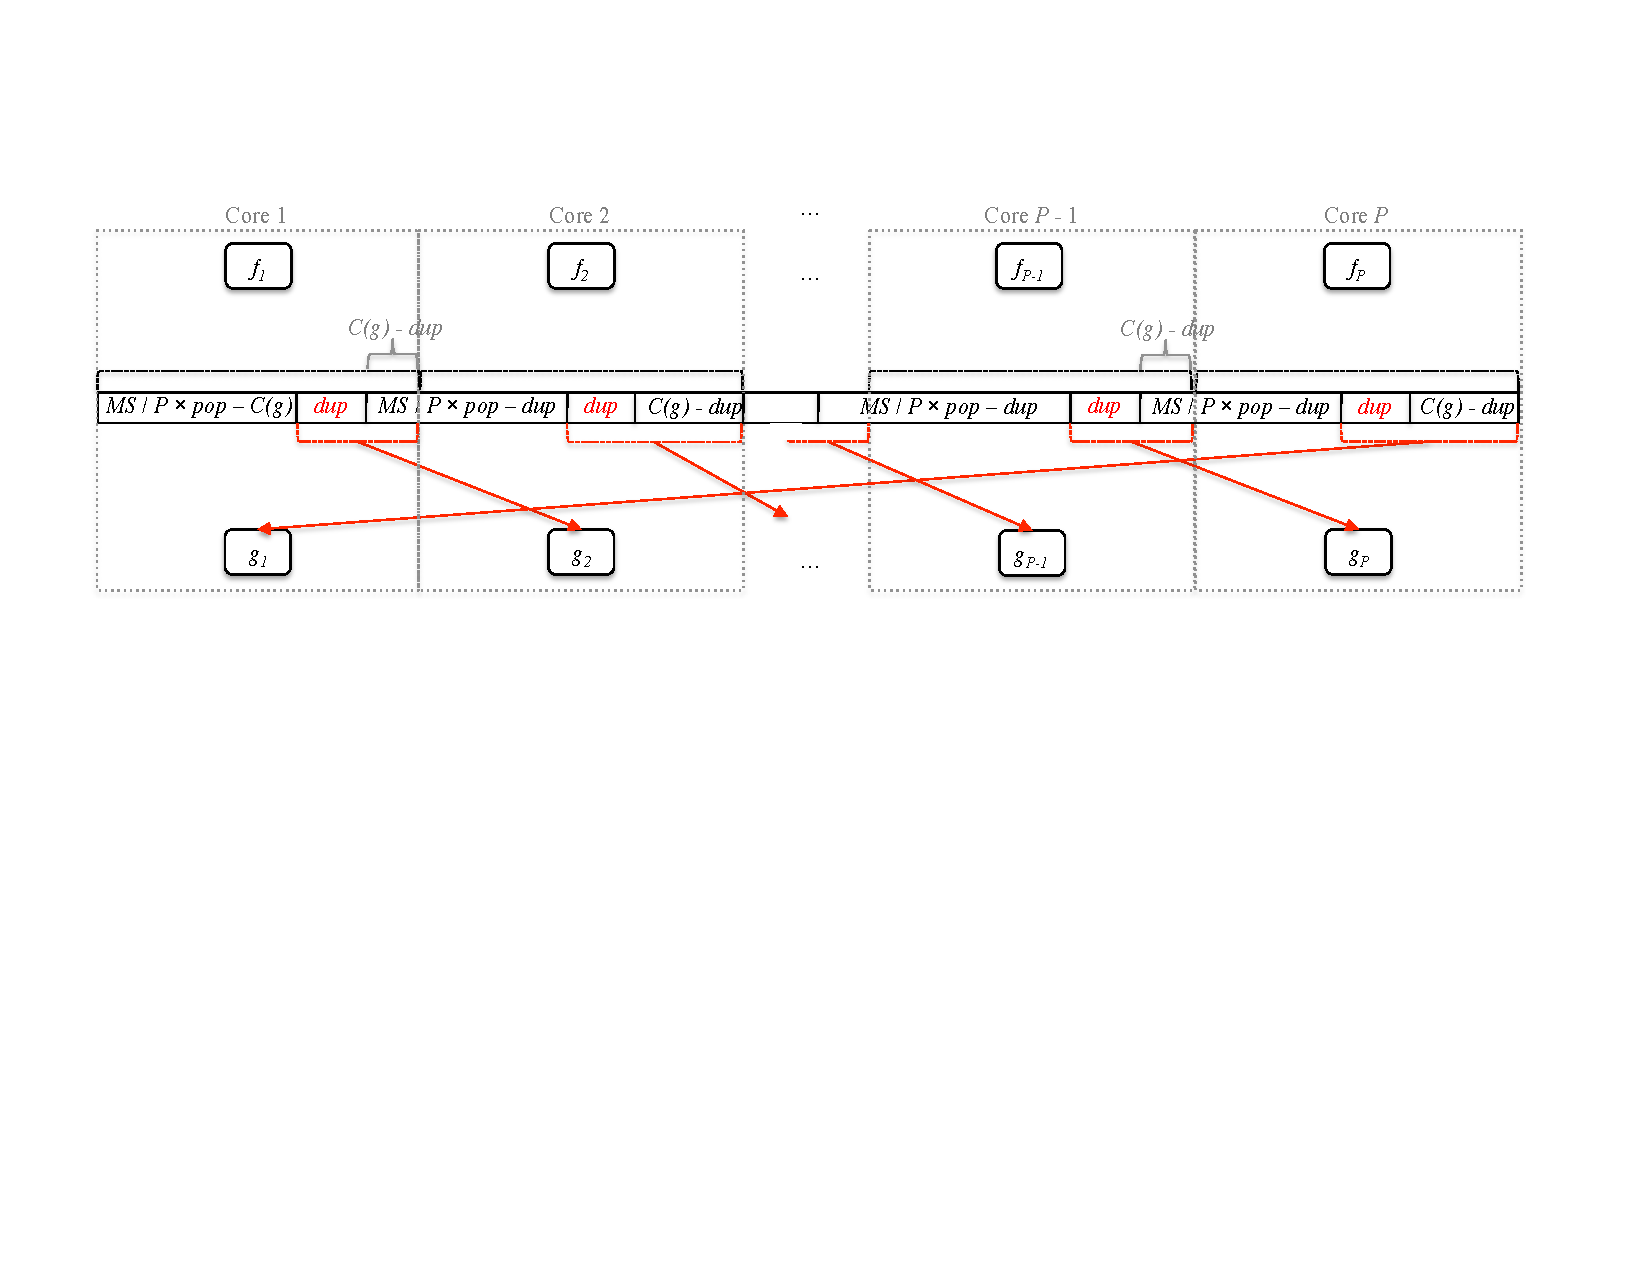
\includegraphics[width=6in]{figures/remaining-dup-case.pdf}
\caption[Extra inter-core communication when $C(g) > \mt{dup}_g$.]
{Inter-core communication details for fission products of consumer $f$
  and producer $g$ each fissed by $P$.  $f$ was a single output node,
  and $g$ was a single input node.  For $g$, $C(g) > \mt{dup}_g$.
  Each $f_i$, $g_i$ pair are mapped to the same core.  The sizes of
  the buffer sections are in terms of $g$. Red arrows denote
  inter-core communication.  \label{fig:remaining-dup}}
\end{figure*}

Figure~\ref{fig:remaining-dup} illustrates the details of
communication between $f$ and $g$ when each is fissed by $P$ with each
$f_i$ mapped to a distinct core, and to the same core as $g_i$.  From
the figure, notice that $C(g)$ items are communicated from $f_i$ to
$g_{i+ 1}$, with $f_P$ sending to $g_1$.  Of the $C(g)$ items,
$\mt{dup}_g$ items are required by both $g_i$ and $g_{i+1}$.  This
corresponds to the orignal number of input items of $g$ that were
inspected by not dequeued for one firing of $g$.  The remaining items,
$C(g) - \mt{dup}_g$, are required to be transfered from $f_i$ to
$g_{i+1}$ when $C(g) > \mt{dup}$ because of misalignment of the items
produced by $f_i$ and required by $g_i$.

When the fission products are assigned to
cores as given in the figure, the percentage of inter-core
communication to total communication can be quantified as:

\begin{equation}
%b\vspace{-2pt}
\label{eq:min-dup}
\mt{InterCore}(g) = \frac{C(g)}{M(S,g) / P * o(W, g)}
%\vspace{-4pt}
\end{equation}

\noindent This percentage corresponds to inter-core communication
ratio for each product filter and, since all product filters have the
same rates, for the total inter-core communication required for the
fission of $g$.

This section covers a technique that seeks to decrease the percentage
of total communication that must be communicated inter-core.  The
technique directly decreases the number of items that are shared,
while also increasing the alignment of communication to minimize
inter-core communication.

Since streaming applications typically execute for many iterations of
the steady-state, it is legal to increase the steady state by $c$.  As
long as this constant $c$ is less than the number of steady-state
iterations $I$ of the application, and $c$ is a factor of $I$.

By recognizing this property, we can directly reduce the amount of
inter-core communication that occurs between the fission products of a
fissed peeking filter for many cases of general fission, including the
common case.  In Equation~\ref{eq:min-dup} we can directly control the
steady-state multiplicity of $g$, $M(S,g)$.  We can calculate a
constant $c_g$ such that the percentage is less than a threshold
$T_{\mt{sharing}}$:

\begin{equation}
\label{eq:ic-thresh}
c_g = \frac{1}{T_{\mt{sharing}}} \cdot \frac{C(g) \cdot P}{M(S,g) \cdot o(W,g)}
\end{equation}

\noindent where $0.0 < T_{\mt{sharing}} \le
\mt{InterCore(g)}$. Increasing the steady-state of the graph by $c_g$
before general fission is applied will assure that the percentage of
items duplicated will be equal to $T_{\mt{sharing}}$.  Sharing
reduction works by increasing the ratio of number of items that are
only needed by one product to the number of items that are needed by
two products.  When we increase the steady-state, in
Figure~\ref{fig:remaining-dup}, the shared (red) sections of the input
buffer to $g$ remain fixed in size, while the private sections of the
input buffer (black) grow.

\subsection{Sharing Reduction for Other Fission Cases}

The sharing reduction optimization does not apply as simply to all
cases of fission of a peeking filter.  Consider the case where we have
single output producer $f$ and single input consumer $g$ with $(f,g)
\in E$, but $f$ and $g$ are fissed by differing widths, i.e., $P_f \ne
P_g$.  This case engenders inter-core communication not only because
of sharing but because of the communication required by the differing
fission widths.  

Going forward, let us assume that $P_f > P_g$.  If $P_f$ is a multiple
of $P_g$, the analysis is straightforward: the percentage of
inter-core communication to total communication is $(1 -
\frac{P_g}{P_f}$). If $P_f$ is not a multiple of $P_g$ misalignment
also occurs because for one or more $g_j$, it's input does not begin
in alignment with any $f_i$'s.  The analysis of the percent of
inter-core communication for this latter case is complex, but it
suffices for our purposes to bound it by $(1 - \frac{P_g}{P_f})$.

Also consider the case where $g$ has multiple inputs. In this case $g$
receives $\mt{RI}(f, g, S) \cdot M(S, g) \cdot o(W,g)$ items from $f$
during the steady-state, and $(1 -\mt{RI}(f, g, S) \cdot M(S, g) \cdot
o(W,g))$ from its other producers. There is a choice: for which
producer of $g$ to optimize the communication of $g$? If $f$ is
chosen, then the assignment of filters to cores should minimize the
inter-core communication by co-locating the fission products of $f$
and $g$ just as the assignment would when $g$ is single input.
However, the calculation must now account for the inter-core
communication of the other producers sending to the fission products
of $g$. 

Now, considering both cases above, we define $\mt{InterCore}(g, f)$ to
approximate the percentage of inter-core communication to total
communication for the input of the fission products of $g$ optimizing
for the placement of the fission products of $f$:

\begin{equation}
\label{eq:tcomm-fopt}
 \mt{InterCore}(g, f)   =  (1 -\mt{RI}(f,g, S) \cdot \frac{P_g}{P_f})
 + \frac{P_g \cdot C(g)}{M(S, g) \cdot o(W, g)}
\end{equation}

\noindent The first term approximates the inter-core communication due
to (i) the fission factor discrepancy between $f$ and $g$, and (ii) the
multiple inputs of $g$.  The second term quantifies the percentage of
inter-core communication caused by the sharing due to peeking.

Increasing the steady-state will not alter the first term of
Eq.~\ref{eq:tcomm-fopt}.  However, the second term can be reduced
because a smaller percentage of steady-state items needs to be
duplicated.  By Amdahl's law, increasing the steady-state can only
decrease $\mt{InterCore}(g, f)$ to under $T_{\mt{sharing}}$ if the
second term of Equation~\ref{eq:tcomm-fopt} accounts for more than
$(1-T_{\mt{sharing}} )$ of the duplication.  

We need to prevent the application of increasing the steady-state to a
filter $g$ that will not benefit from it because the majority of
inter-core communication from fission of $g$ is not caused by $g$'s
sliding window.  We define a constant $T_{\mt{apply}}$ such that
sharing reduction should only be applied to $g$ optimizing for $f$ if:

\begin{equation}
\label{eq:apply-sharing}
T_{\mt{sharing}}  >  T_{\mt{apply}} \ge (1 -\mt{RI}(f,g, S) \cdot
\min(\frac{P_g}{P_f}, \frac{P_f}{P_g}))
\end{equation}

% \begin{equation}
% T_{\mt{sharing}}  >  T_{\mt{apply}} \ge (1 -\mt{RI}(f,g, S) \cdot
% \frac{P_g}{P_f})
% \end{equation}

\noindent Since it was first assumed that $P_f > P_g$, in order to
generalize we must choose the appropriate fraction of local
communication by taking the minimum of the two fission width ratios.

In the common case where $f$ and $g$ are fissed by the same width, and
$f$ has single output and $g$ has single input, the RHS of
Eq.~\ref{eq:apply-sharing} evaluates to 0, indicating to always apply
sharing reduction.  If however, the RHS of Eq.~\ref{eq:apply-sharing}
does not evaluate to 0, there exists inter-core communication that is
not attributed to sliding windows.  In this latter case,
$T_{\mt{apply}}$ determines at what percent of total inter-core
communication, non-sliding-window inter-core communication should
prevent the application of sharing reduction.  For example, if
$T_{\mt{apply}} = .05$, then we will apply sharing reduction only when
sliding window inter-core communication accounts or at least 95\% of
total inter-core communication for the proposed fission application of
$g$. $T_{\mt{apply}}$ prevents the application of sharing reduction to
fission when the bulk of inter-core communication of the fission is
not caused by sliding windows, and thus will not be reduced by
increasing the steady-state.

% For simplicity of analysis, let us assume that $C(g)
% = 0$, and $P_f$ is a multiple of $P_g$. Figure~\ref{fig:diff-widths}
% presents an example with these assumptions.  In the example, $f$ and
% $g$ are fissed by 8 and 4 respectively.  Since we want to maintain
% data parallelism, each $f_i$, $1 \le i \le P_f$, is mapped to a
% distinct core, as is each $g_j$, $1 \le j \le P_g$.  Since each $f_i$
% produces half the number of items required by each $g_j$, half the
% communication in this case is inter-core, caused by the misalignment
% of the rates of the producer and consumer fission products.


% Additionally, if $C(g) > 0$, it is required to share $C(g)$ items
% between two cores.  There are $P_g$ sections of $C(g)$ items, and this
% data has to be communicated inter-core to one other core.  Given this
% analysis, we can quantify an {\it approximation} of the percentage of
% inter-core communication for the fission application of $g$ when $P_f
% > P_g$:

% \begin{align}
% \mt{InterCore}(g) & = & \frac{(1 - \frac{P_g}{P_f}) \cdot M(S, g) \cdot o(W, g) +
% P_g \cdot C(g)}{M(S, g) \cdot o(W, g)} \\
% \label{eq:diff-fiss}
% \mt{InterCore}(g) & = & (1 - \frac{P_g}{P_f}) +
% \frac{P_g \cdot C(g)}{M(S, g) \cdot o(W, g)}
% \end{align}

% The first term on the RHS of Equation~\ref{eq:diff-fiss} gives the
% percentage of inter-core communication produced by the fission width
% inequality.  

% \begin{equation}
% \label{eq:tcomm-fopt1}
%  \mt{InterCore}(g,f)   = (1 - \mt{RI}(f,
%    g, S))  + (1 - \frac{P_g}{P_f}) \cdot \mt{RI}(f,
%    g, S)   + \frac{P_g \cdot C(g)}{M(S, g) \cdot o(W, g)} 
% \end{equation}

% \noindent The first term accounts for the percentage of items that $g$'s fission
% products receive from producers that are not products of $f$.  The
% second term, the percentage items that are communicated inter-core
% because of the fission width mis-alignment, must now account for the
% fact that not all items are from $f$.  Equation~\ref{eq:tcomm-fopt1}
% can be simplified to:


\subsection{Sharing Reduction Applied to the Stream Graph}
So far we have considered the application of the sharing reduction
optimization to a single filter $g$ in the stream graph.  Now we will
cover how to apply sharing reduction across all the filters of the
stream graph for which it is appropriate.  The goal is reduce the
percentage of inter-core communication due to the sharing between
fission products of all peeking filters to {\it approximately}
$T_{\mt{sharing}}$ of total inter-core communication for the fission
of all peeking filters.  Sharing reduction may not achieve
$T_{\mt{sharing}}$ because there may exist peeking filters that are to
be fissed for which Equation~\ref{eq:apply-sharing} cannot be
satisfied.  For these filters, we do not apply the sharing reduction
optimization.

The process of applying sharing reduction to the entire stream graph
consists of determining which filters are appropriate and determining
a steady-state multiplier by which to increase the graph.  To
determine the steady-state graph multiplier, the compiler calculates
the percentage of sharing over all of the filters which adhere to
Equation~\ref{eq:apply-sharing}.  Let $\Phi$ denote the set of filters
for which Equation~\ref{eq:apply-sharing} holds and that we seek to
fiss:

\begin{equation}
\label{eq:sr-mult}
c = \frac{1}{T_{\mt{sharing}}} \cdot \frac{\sum_{g \in \Phi} P_g \cdot C(g) }{\sum _{g \in
    \Phi} M(S, g) \cdot o(W, g)}
\end{equation}

\noindent Increasing the steady-state by $c$ for all filters of the
graph will reduce the total sharing for the filters of $\Phi$ to
$T_{\mt{sharing}}$.  




% In the
%  graph before fission is applied, $C(g)$ items will remain in the
%  input buffer of $g$ between steady-state iterations.  After fission by $P$,
%  for each steady-state, $g_1$ will first consume the $C(g)$ items that
%  $f_p$ sent it from the previous steady-state iteration.  $g_1$ will
%  then require:

% \[ M(S, g)/P \cdot o(W, g) + \mt{dup} - C(g)\]

% \noindent additional items from $f_1$.\footnote{It is guaranteed that
%   $M(S, g)/P \cdot o(W, g) > C(g)$ by the precondition of general
%   fission.} This requirement is less than the number of items that
% $f_1$ produces $M(S, g)/P \cdot o(W, g)$ since $C(g) > \mt{dup}$. So,
% $C(g) - \mt{dup}$ items must be transferred from $f_1$ to $g_2$ in
% addition to the shared and duplicated $\mt{dup}$. In all, $C(g)$ items
% must be transferred from $f_i$ to $g_{i+1}$.

%  Each $f_i$ produces $M(S,f)/p
% \cdot u(S,f)$ items, while each $g_i$ must consume the original pop
% rate multiplied by it's slice of $f$'s multiplicity plus the number of
% inspected items of $g$:

% \[ M(S,g)/P \cdot o(W, g) + C(g) \]

% \noindent Since $M(S,g)/P \cdot o(W, g) = M(S,f)/p
% \cdot u(S,f)$, the number of items each $f_i$ produces and the number
% of items each $g_i$ consumes differs by $C(g)$.
% As Figure~\ref{fig:core-comm} demonstrates, each $g_i$
% receives $C(g)$ duplicated items from $g_{i-1}$ (with $g_1$
% receiving from $f_p$).  
